%=== Préambule ===========================================================

\documentclass{beamer}
\usepackage{pdfpages}
\usepackage[english]{babel}
\usepackage{xspace}
\usepackage{pifont}
\usepackage{hyperref}
\usepackage{listings}
\usepackage{csquotes}
\usepackage{graphicx}
\usepackage{animate,media9} %,movie15}
\usepackage{wrapfig}
\usepackage{pdfpages}
\usepackage{tikz}
\usepackage{natbib}
\uselanguage{English}
\usepackage{fontawesome5}
\languagepath{English}
\setcounter{tocdepth}{1}
\usepackage{setspace}
\usepackage{amsmath}
\def\glasses{{\sffamily 
\leavevmode\rlap{%
\rotatebox[origin=tr]{125}{J}\kern1ex%  
\rotatebox[origin=tr]{125}{J}}% 
\rotatebox[origin=c]{-90}{D}%   
\rotatebox[origin=c]{-90}{D}}%
\def\ialy{\sffamily 
\resizebox{1ex}{1.5ex}{\reflectbox{\rotatebox[origin=]{75}{J}}}\kern-1pt%
\rlap{\tiny$\ ^\bullet\kern2.5pt^\bullet$ }%
\rotatebox[origin=c]{-90}{D}%   
\rotatebox[origin=c]{-90}{D}\kern-1pt%  
\resizebox{1ex}{1.5ex}{\rotatebox[origin=]{75}{J}}}}


\lstset{
  numbers=left,
  basicstyle=\tiny\ttfamily,      
  breaklines=true, 
  showtabs=false,
  showstringspaces=false,
}  

%=== Configuration de Beamer et du thème metropolis ======================
\usepackage{bbding}
\usetheme[background=light]{metropolis}
\usepackage[clock]{ifsym}

\definecolor{mLightBrown}{HTML}{000000}
\definecolor{black}{HTML}{000000}
\setbeamercolor{structure}{fg=black,bg=mLightBrown}
\setbeamercolor{palette primary}{%
	use=normal text,
	fg=normal text.bg,
	bg=mLightBrown
}
%\setsansfont[BoldFont={Linux Libertine G Bold},Numbers={OldStyle}]{Linux Libertine G}

\metroset{block=fill}

%=== Page de titre =======================================================

%path to logo and biblio -> to be adapted to your local directories 
\newcommand\dirlogo{../../logos/}
\newcommand\dirbiblio{../../biblio}



\title{{\normalsize \vskip 1cm Exploring complex normal faulting systems through physics-based dynamic rupture modeling}}
\subtitle{\small }
\author{Hugo S. \\ {\tiny Institut de Recherche pour le Développement IRD - ISTerre} \\ 
\\
O., Scotti, S., Hok, A.-A. Gabriel and T. Taufiqurrahman \\
\\
\textit{ANR EQTIME Project}
}


\date[2021]{\today}

\subject{Group Meeting}

\titlegraphic{\centering \vspace{-15pt}
\includegraphics[height=1.3cm]{../../logos/logo_all_presentation.pdf} \par} %\qquad  
\includegraphics[height=1.4cm]{../../logos/anr_eqtime.png} \par }


\addtobeamertemplate{frametitle}{}{%
\begin{tikzpicture}[remember picture,overlay]
  \node[anchor=north east,yshift=0.0ex] at (current page.north east) {
\includegraphics[height=4ex]{../../logos/ISTerre_neg.pdf}};
  %\node[anchor=north east,yshift=0.5ex] at (current page.north east) {\includegraphics[height=3.3ex]{\dirlogo/seiscope_color_light_background}};
\end{tikzpicture}}



%=== Document ============================================================

\begin{document}

% --- Préambule ---------------------------------------------------------------

\begin{frame}
    \titlepage
\end{frame}

\begin{frame}
 {Outline}
 
 \tableofcontents
 
\end{frame}

\begin{frame}
 {Geometry of virtual receivers}

 \centering
 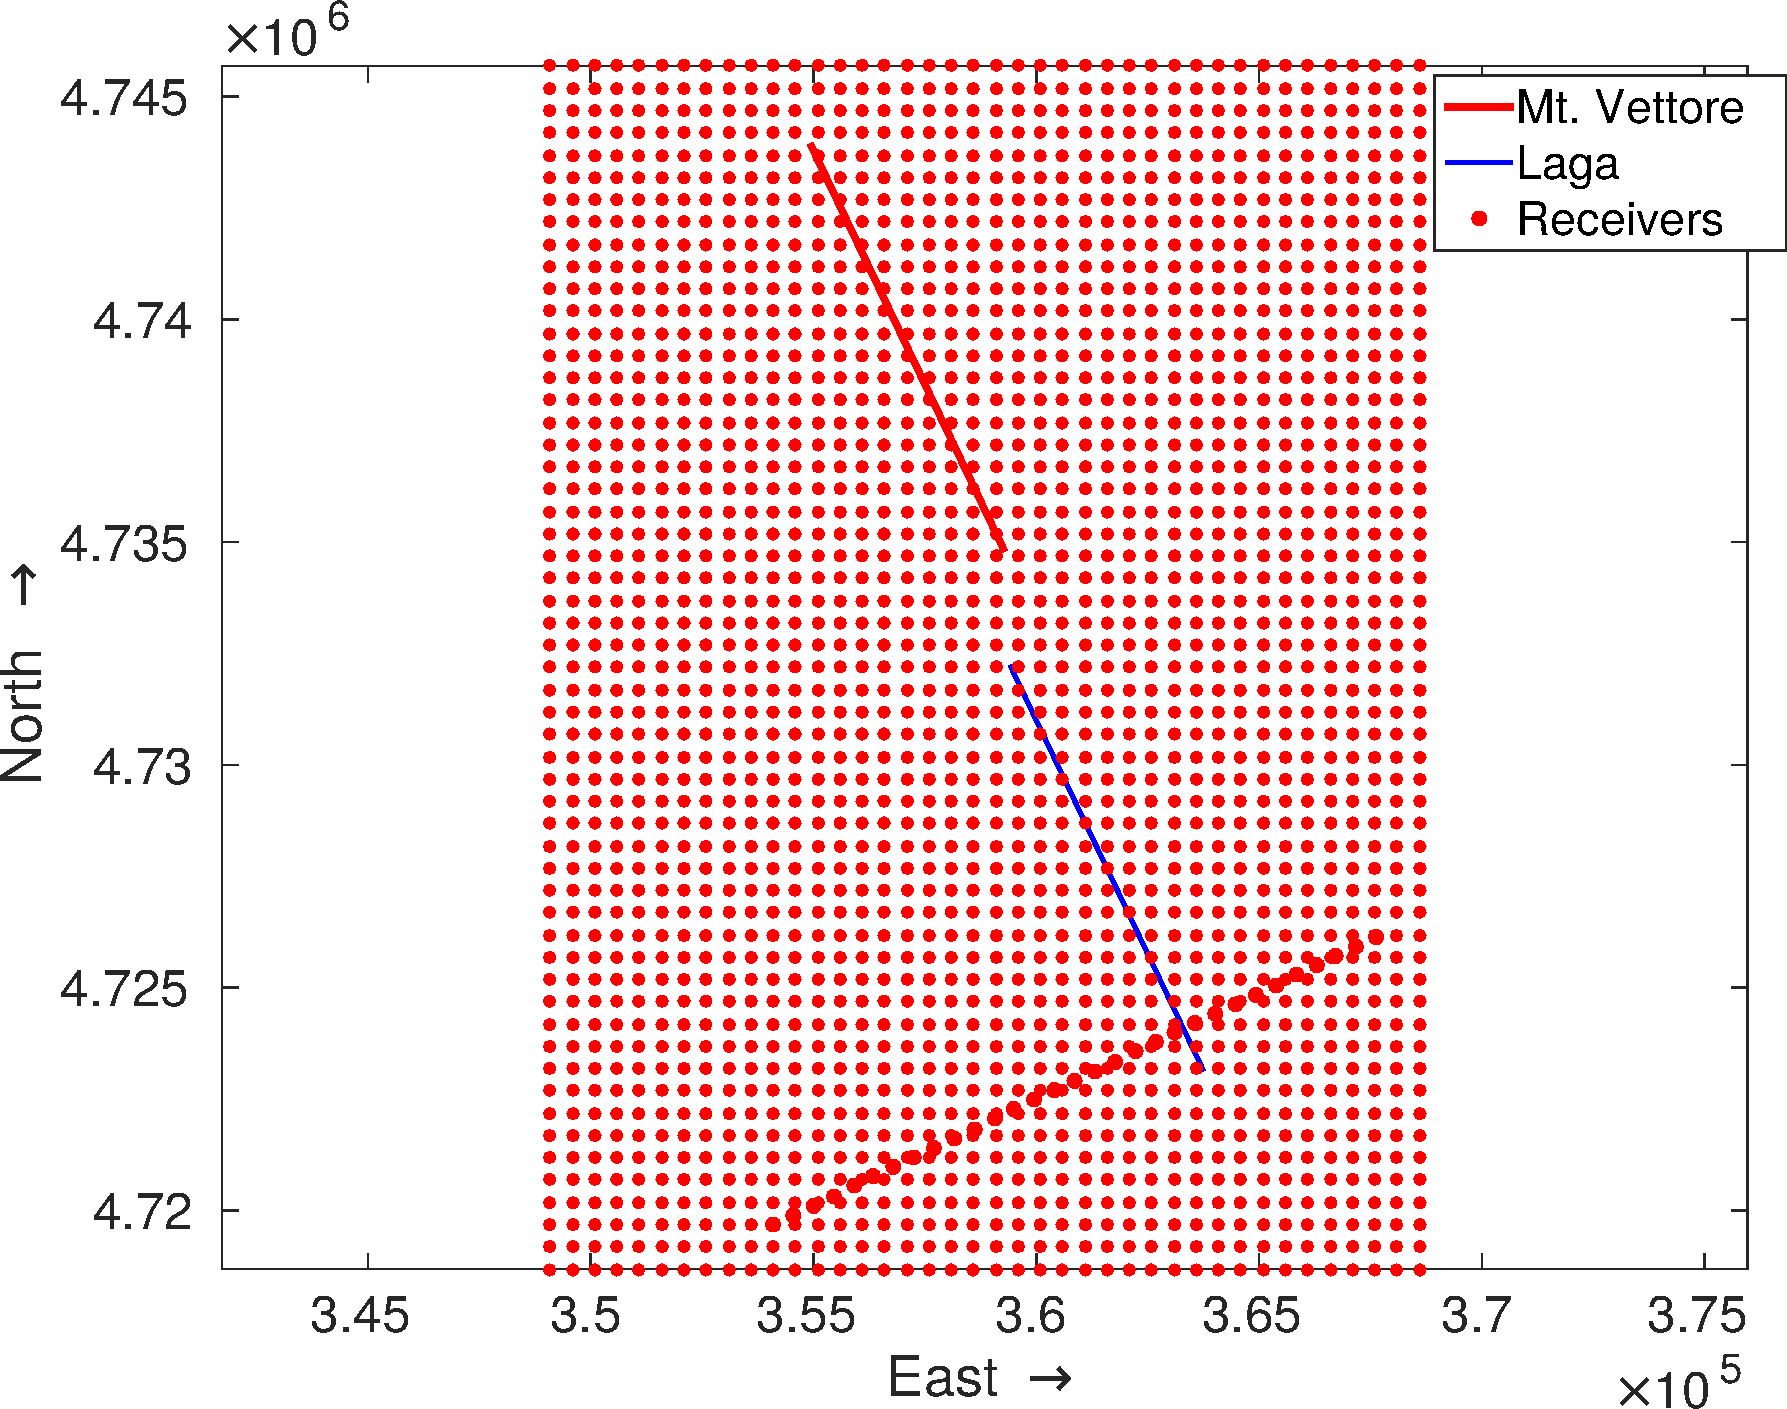
\includegraphics[width=1.1\linewidth]{images/virtual_rec}
 
 \centering offset=2.5 km gap=1.0 km (JUMP)
 
\end{frame}

\begin{frame}
 {Estimation of shear stress}
 
 \centering
 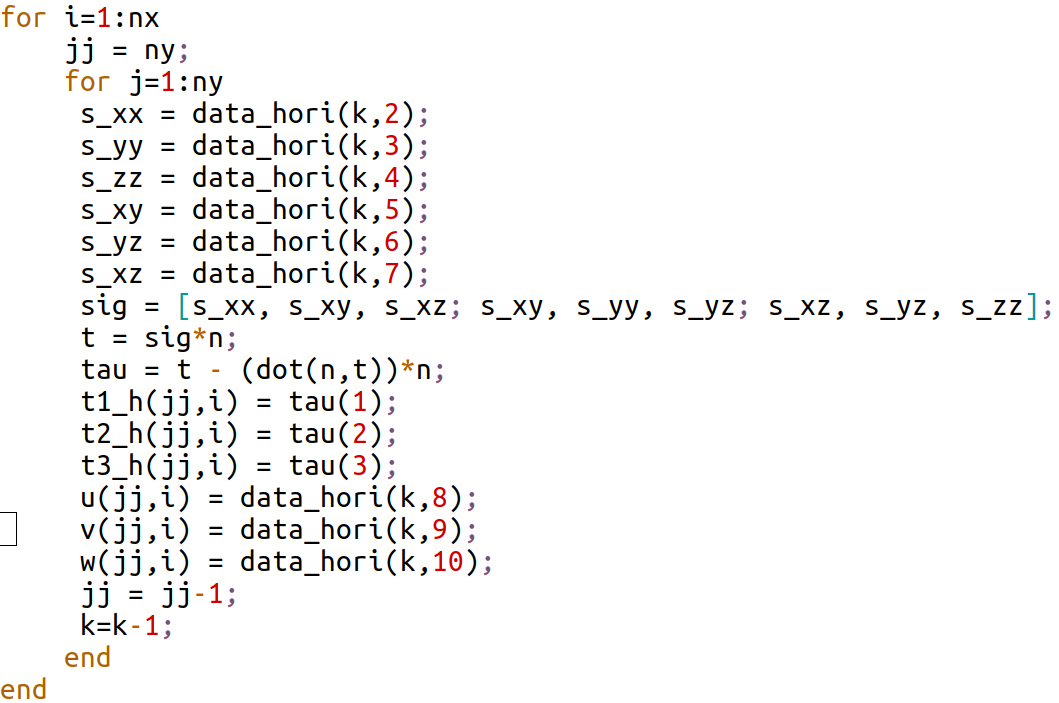
\includegraphics[width=1\linewidth]{images/formula}
 
\end{frame}


\begin{frame}
 {Shear stress}
 
 \centering \Large T = 0 s\\
 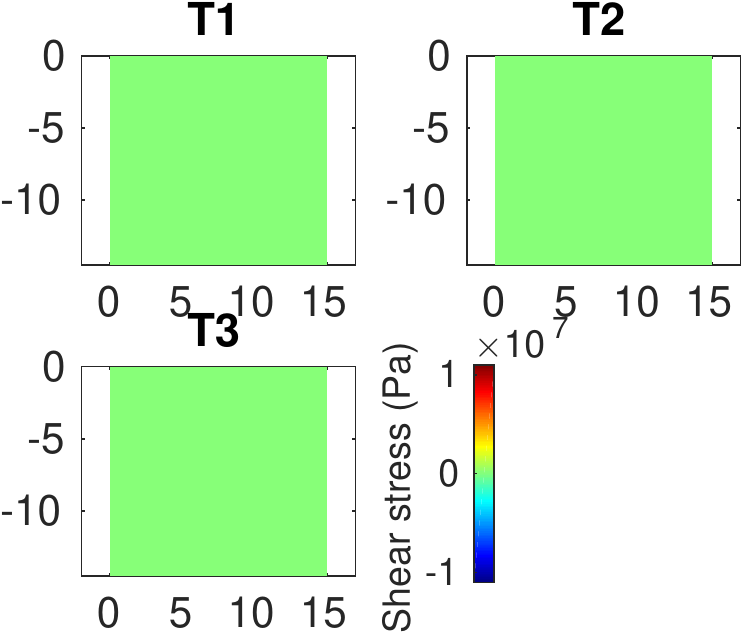
\includegraphics[width=0.8\textwidth]{images/vertical_00006}
 
\end{frame}

\begin{frame}
 {Shear stress}
 
 \centering \Large T = 0.5 s\\
 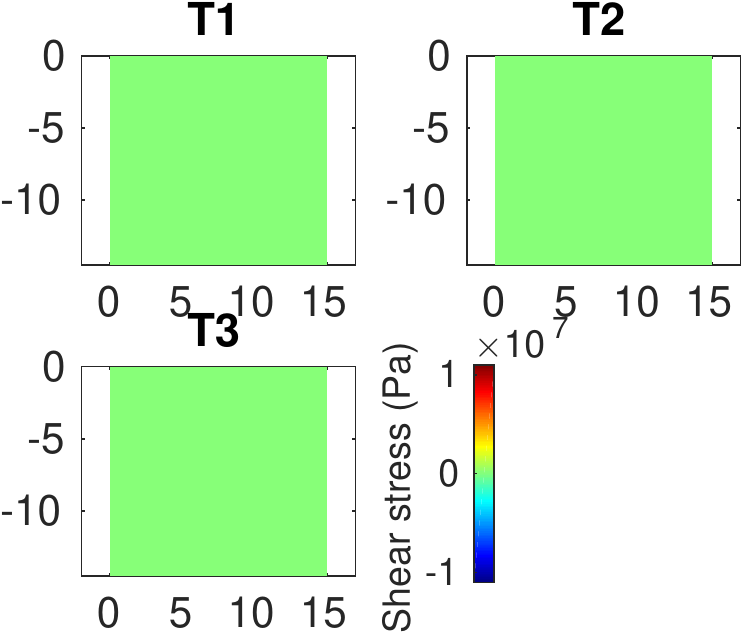
\includegraphics[width=0.8\textwidth]{images/vertical_00011}
 
\end{frame}

\begin{frame}
 {Shear stress}
 
 \centering \Large T = 1 s\\
 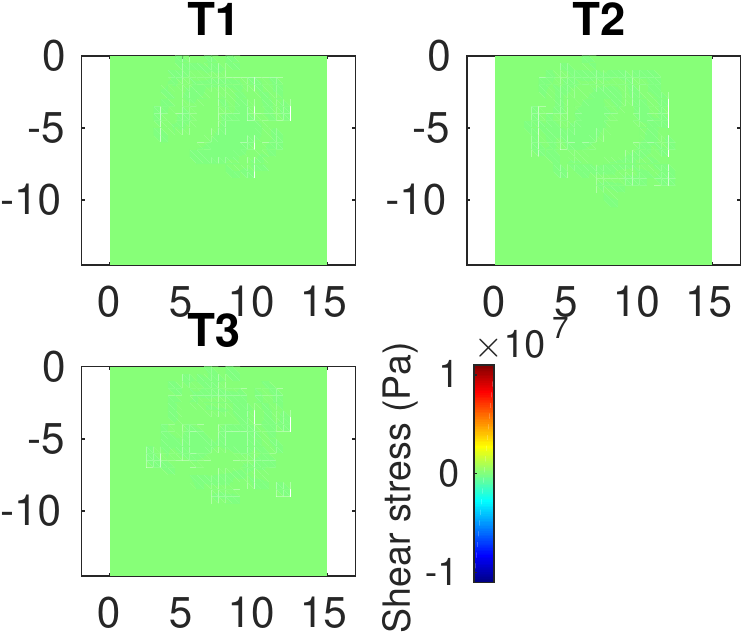
\includegraphics[width=0.8\textwidth]{images/vertical_00016}
 
\end{frame}

\begin{frame}
 {Shear stress}
 
 \centering \Large T = 1.5 s\\
 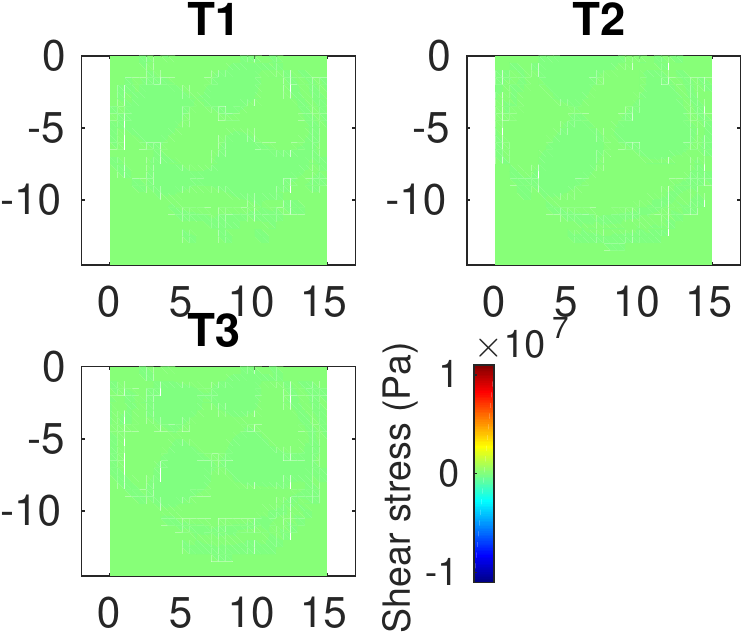
\includegraphics[width=0.8\textwidth]{images/vertical_00021}
 
\end{frame}

\begin{frame}
 {Shear stress}
 
 \centering \Large T = 2 s\\
 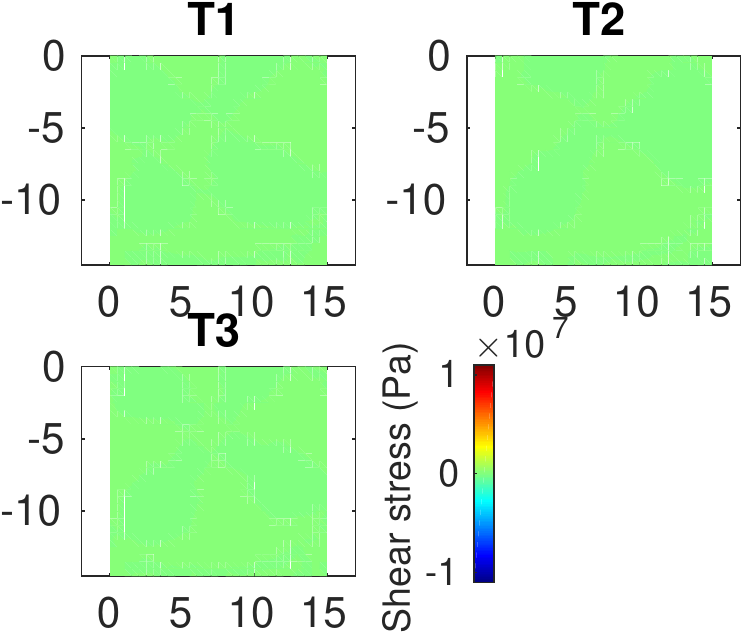
\includegraphics[width=0.8\textwidth]{images/vertical_00026}
 
\end{frame}

\begin{frame}
 {Shear stress}
 
 \centering \Large T = 2.5 s\\
 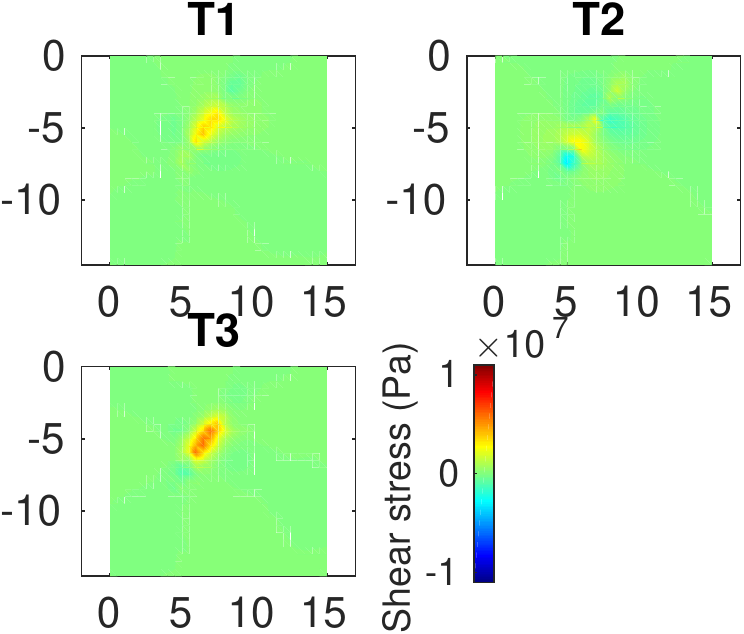
\includegraphics[width=0.8\textwidth]{images/vertical_00031}
 
\end{frame}

\begin{frame}
 {Shear stress}
 
 \centering \Large T = 3 s\\
 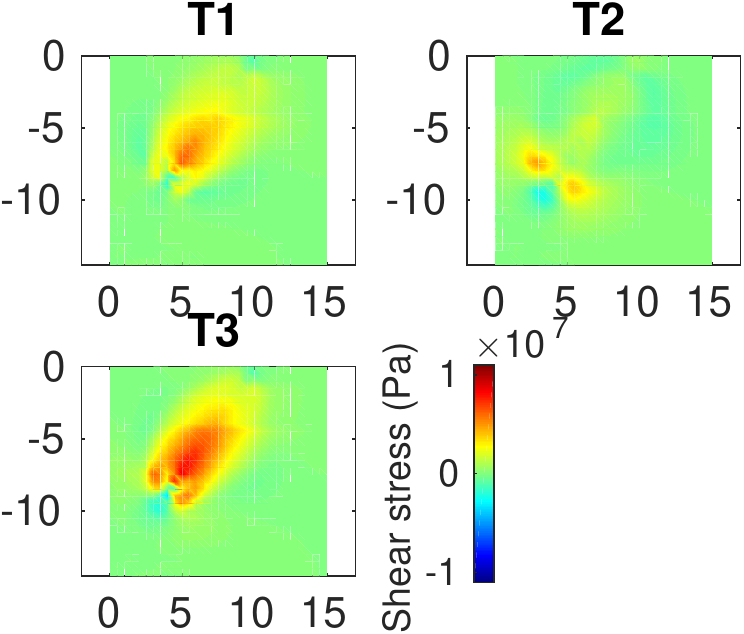
\includegraphics[width=0.8\textwidth]{images/vertical_00036}
 
\end{frame}

\begin{frame}
 {Shear stress}
 
 \centering \Large T = 3.5 s\\
 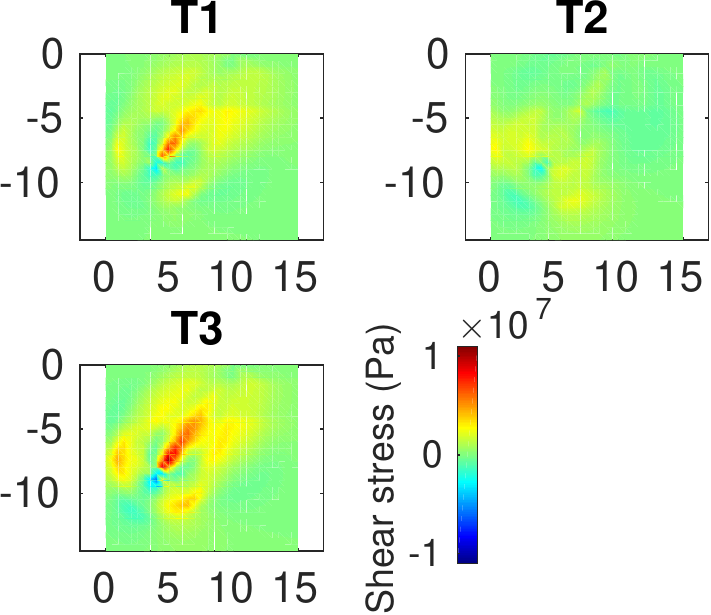
\includegraphics[width=0.8\textwidth]{images/vertical_00041}
 
\end{frame}

\begin{frame}
 {Shear stress}
 
 \centering \Large T = 4 s\\
 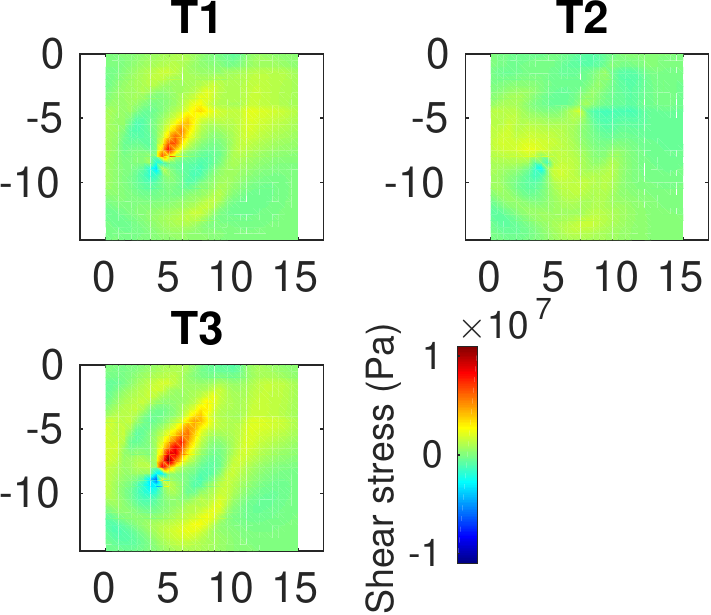
\includegraphics[width=0.8\textwidth]{images/vertical_00046}
 
\end{frame}

\begin{frame}
 {Shear stress}
 
 \centering \Large T = 4.5 s\\
 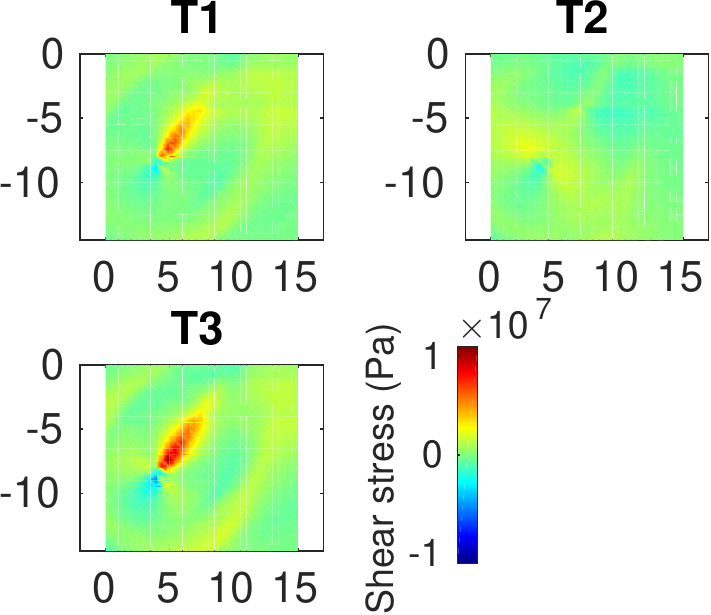
\includegraphics[width=0.8\textwidth]{images/vertical_00051}
 
\end{frame}

\begin{frame}
 {Shear stress}
 
 \centering \Large T = 5 s\\
 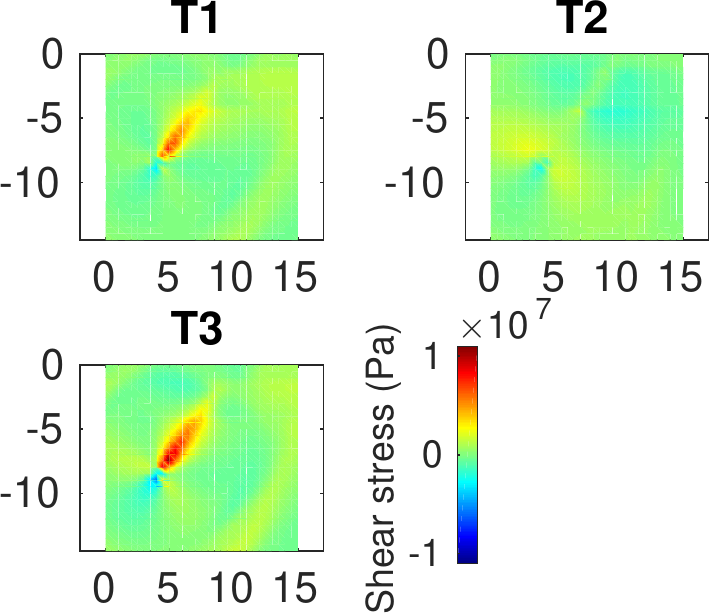
\includegraphics[width=0.8\textwidth]{images/vertical_00056}
 
\end{frame}

\begin{frame}
 {Shear stress}
 
 \centering \Large T = 5.5 s\\
 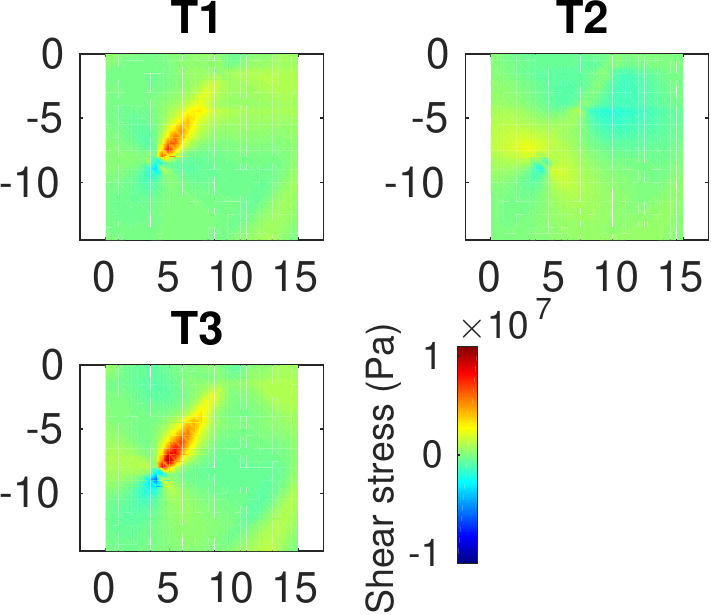
\includegraphics[width=0.8\textwidth]{images/vertical_00061}
 
\end{frame}

\begin{frame}
 {Shear stress}
 
 \centering \Large T = 6 s\\
 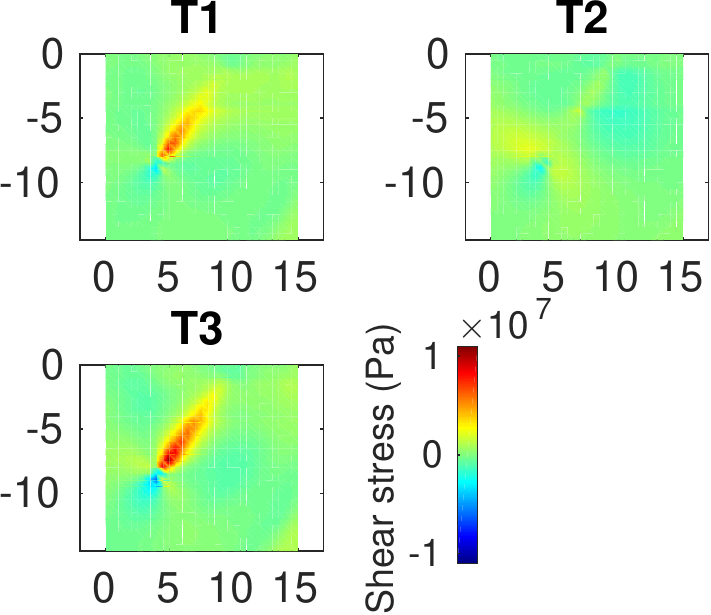
\includegraphics[width=0.8\textwidth]{images/vertical_00066}
 
\end{frame}

\begin{frame}
 {Shear stress}
 
 \centering \Large T = 6.5 s\\
 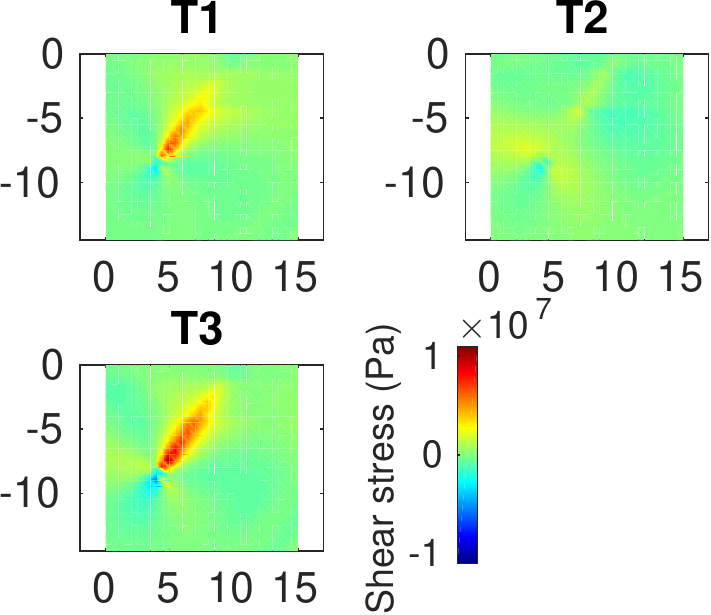
\includegraphics[width=0.8\textwidth]{images/vertical_00071}
 
\end{frame}

\begin{frame}
 {Shear stress}
 
 \centering \Large T = 7 s\\
 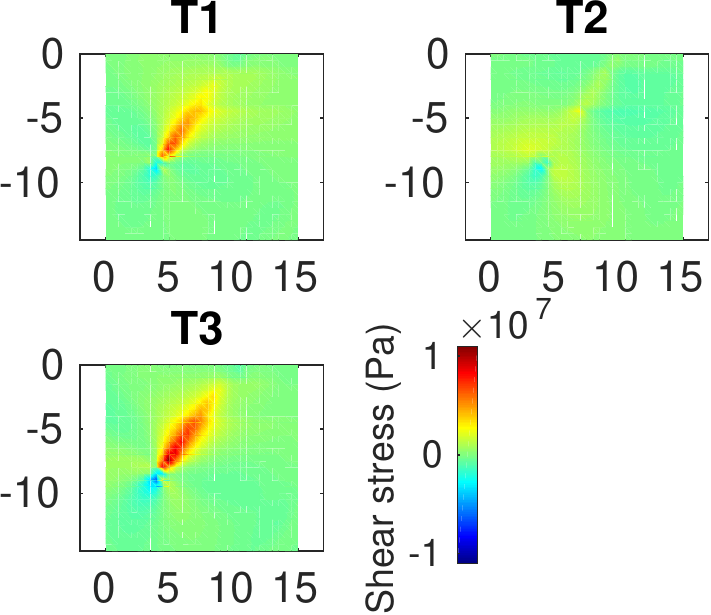
\includegraphics[width=0.8\textwidth]{images/vertical_00076}
 
\end{frame}

\begin{frame}
 {Shear stress}
 
 \centering \Large T = 7.5 s\\
 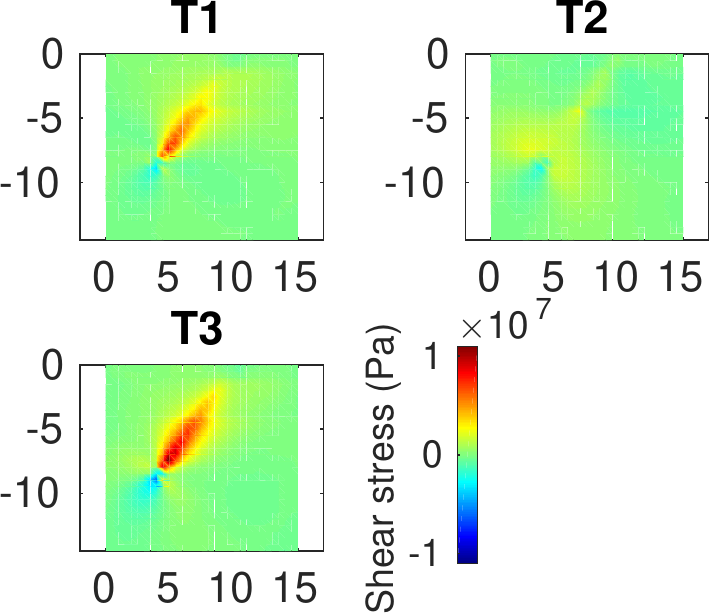
\includegraphics[width=0.8\textwidth]{images/vertical_00081}
 
\end{frame}

\begin{frame}
 {Shear stress}
 
 \centering \Large T = 8 s\\
 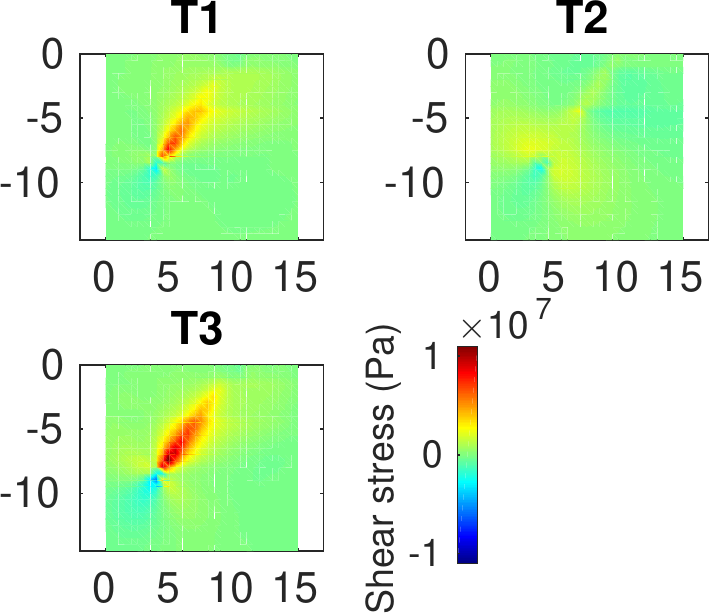
\includegraphics[width=0.8\textwidth]{images/vertical_00086}
 
\end{frame}

\begin{frame}
 {Shear stress}
 
 \centering \Large T = 8.5 s\\
 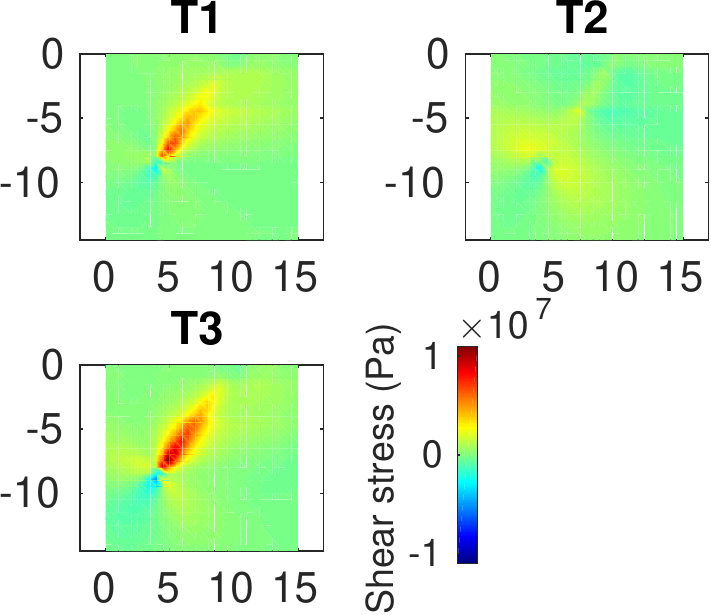
\includegraphics[width=0.8\textwidth]{images/vertical_00091}
 
\end{frame}

\begin{frame}
 {Shear stress}
 
 \centering \Large T = 9 s\\
 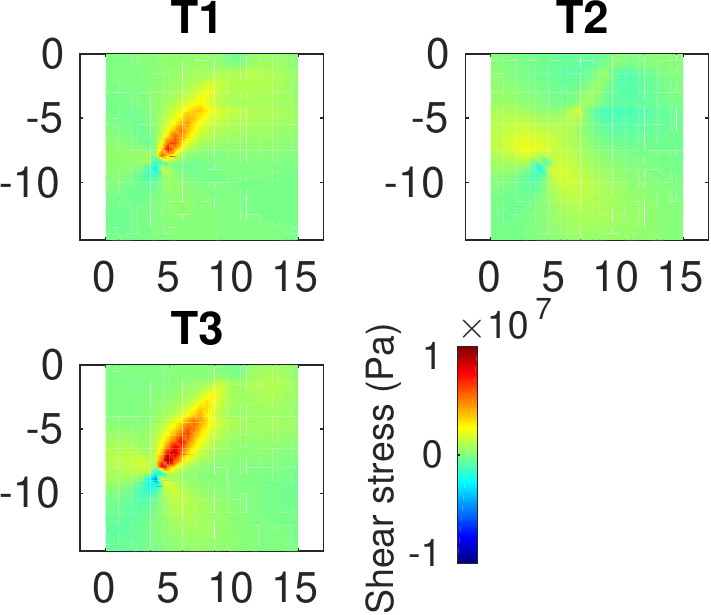
\includegraphics[width=0.8\textwidth]{images/vertical_00096}
 
\end{frame}

\begin{frame}
 {Shear stress}
 
 \centering \Large T = 9.5 s\\
 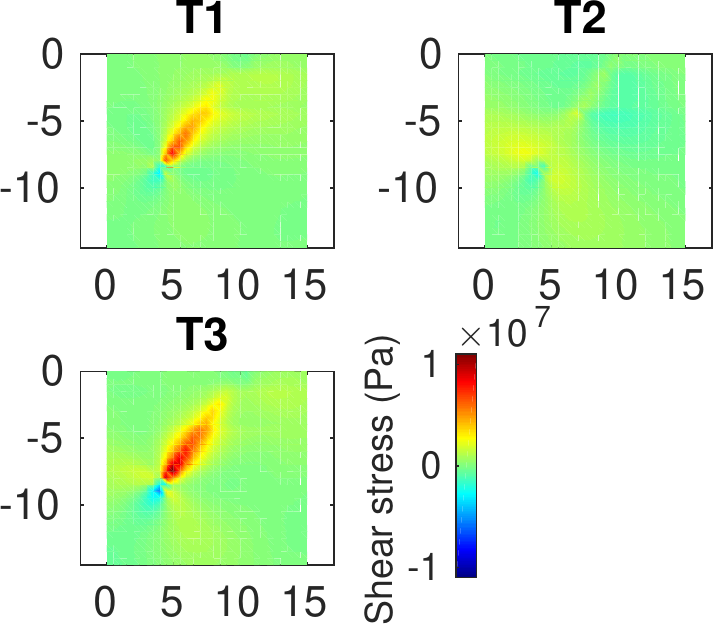
\includegraphics[width=0.8\textwidth]{images/vertical_00101}
 
\end{frame}

\begin{frame}
 {Shear stress}
 
 \centering \Large T = 10 s\\
 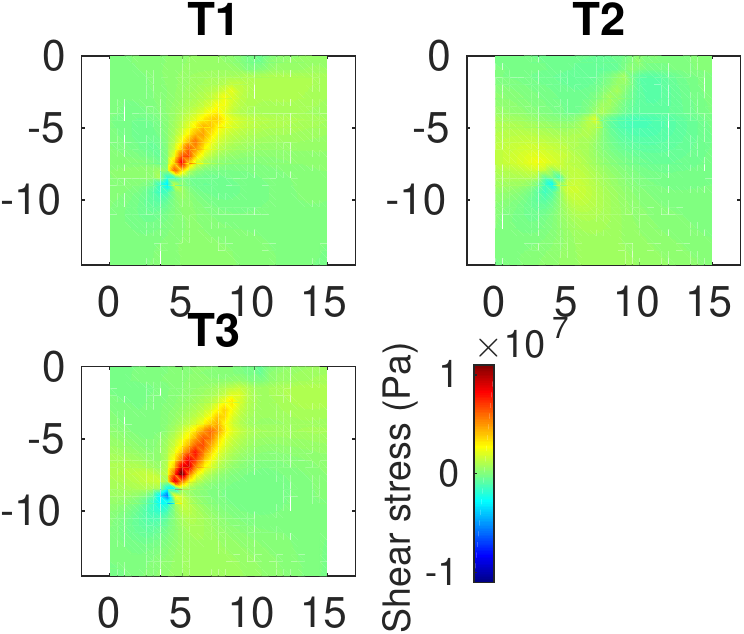
\includegraphics[width=0.8\textwidth]{images/vertical_00106}
 
\end{frame}

\begin{frame}
 {Shear stress}
 
 \centering \Large T = 10.5 s\\
 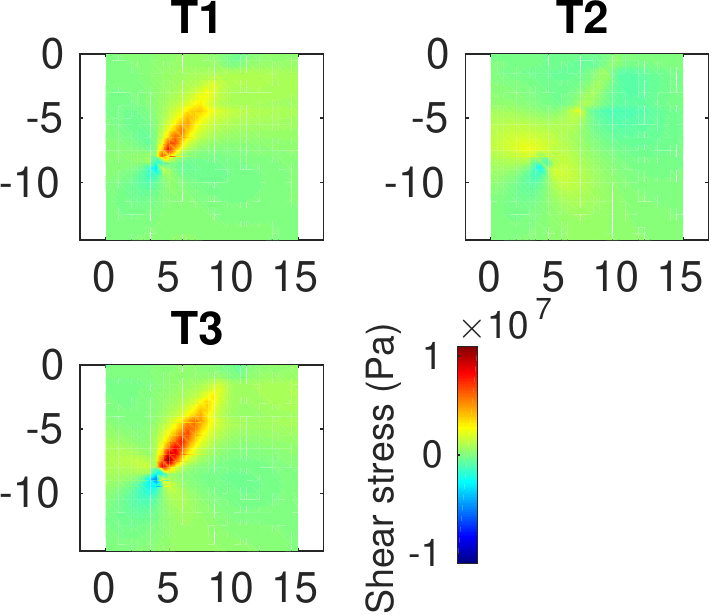
\includegraphics[width=0.8\textwidth]{images/vertical_00111}
 
\end{frame}

\begin{frame}
 {Shear stress}
 
 \centering \Large T = 11 s\\
 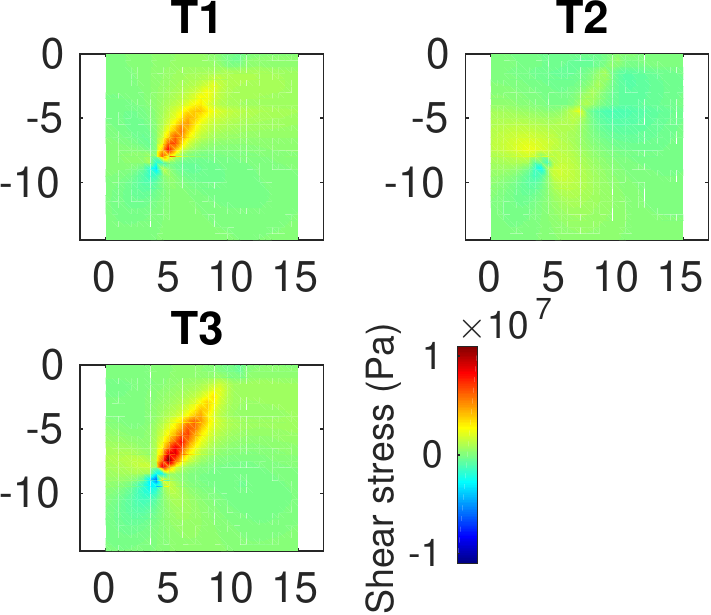
\includegraphics[width=0.8\textwidth]{images/vertical_00116}
 
\end{frame}



\begin{frame}
 {Shear stress}
 
 \centering \Large T = 0 s\\
 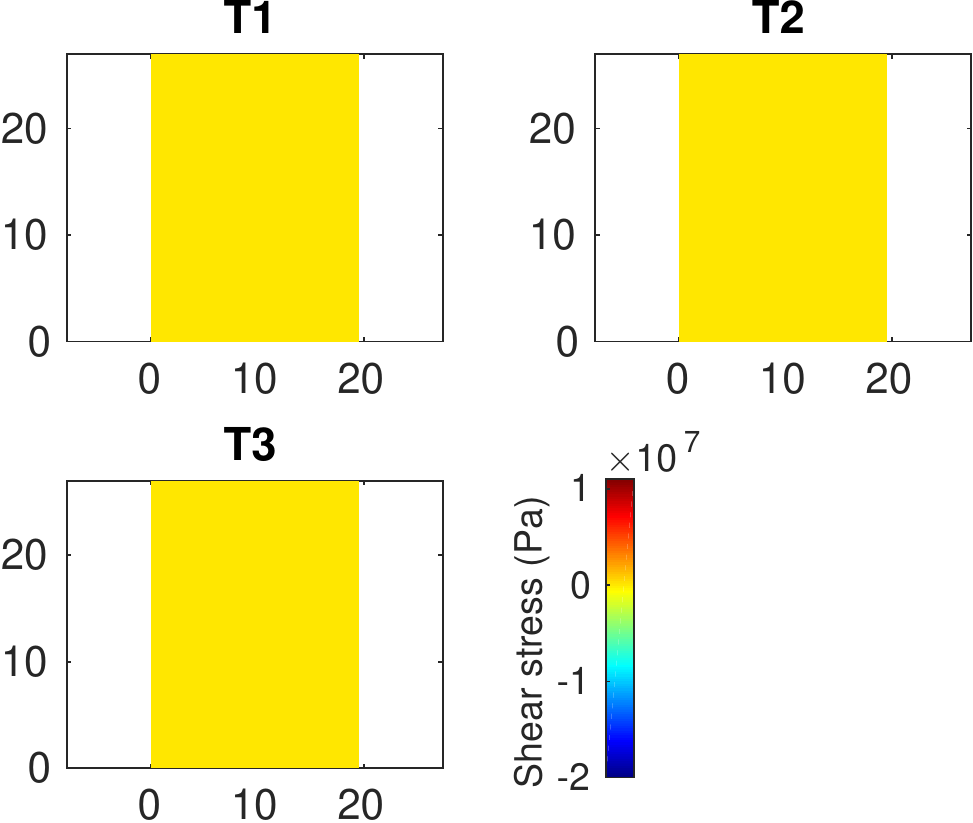
\includegraphics[width=0.8\textwidth]{images/horizontal_00006}
 
\end{frame}

\begin{frame}
 {Shear stress}
 
 \centering \Large T = 0.5 s\\
 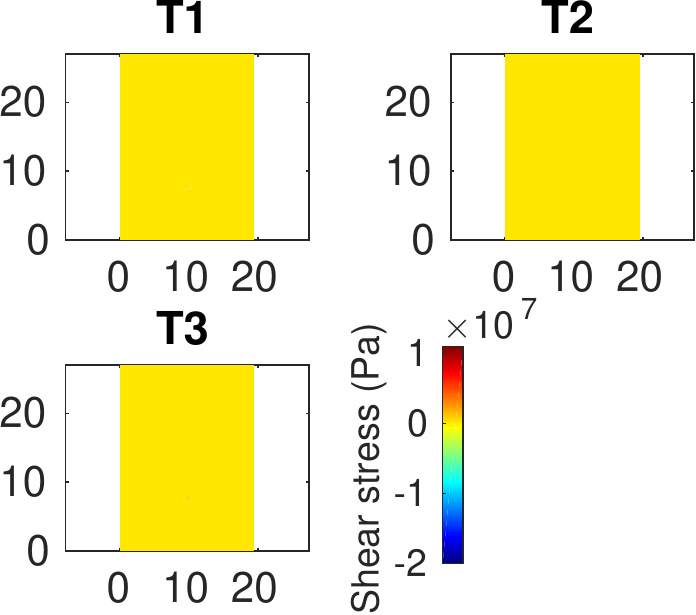
\includegraphics[width=0.8\textwidth]{images/horizontal_00011}
 
\end{frame}

\begin{frame}
 {Shear stress}
 
 \centering \Large T = 1 s\\
 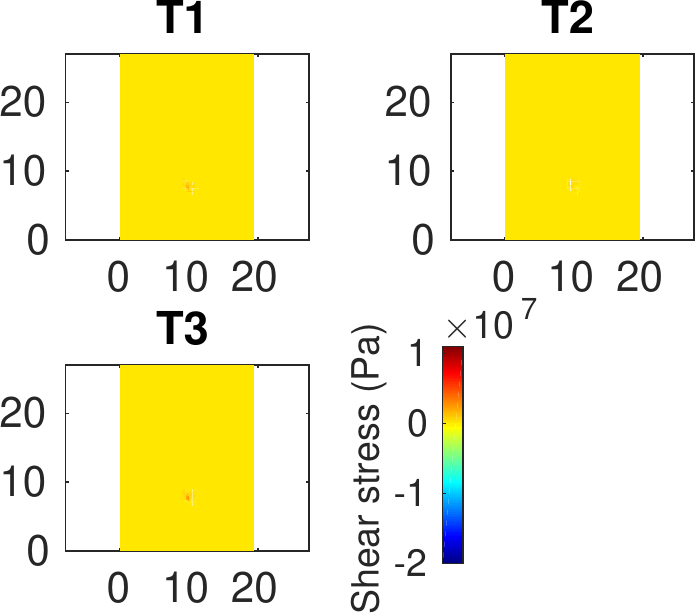
\includegraphics[width=0.8\textwidth]{images/horizontal_00016}
 
\end{frame}

\begin{frame}
 {Shear stress}
 
 \centering \Large T = 1.5 s\\
 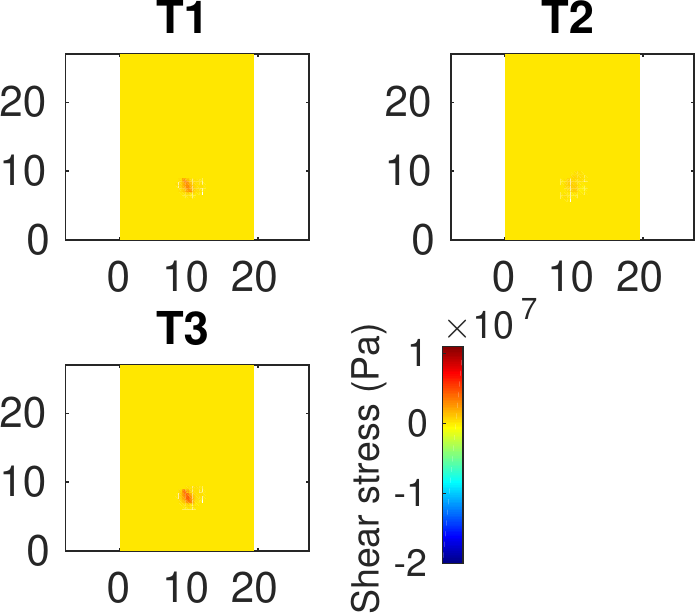
\includegraphics[width=0.8\textwidth]{images/horizontal_00021}
 
\end{frame}

\begin{frame}
 {Shear stress}
 
 \centering \Large T = 2 s\\
 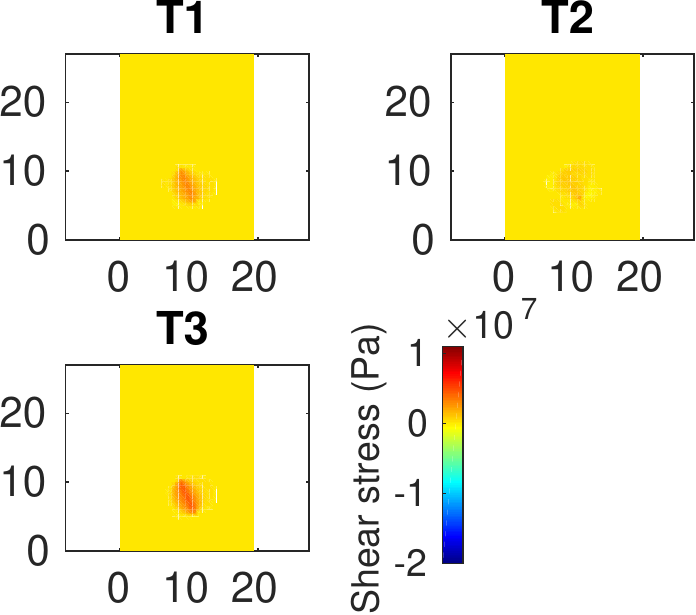
\includegraphics[width=0.8\textwidth]{images/horizontal_00026}
 
\end{frame}

\begin{frame}
 {Shear stress}
 
 \centering \Large T = 2.5 s\\
 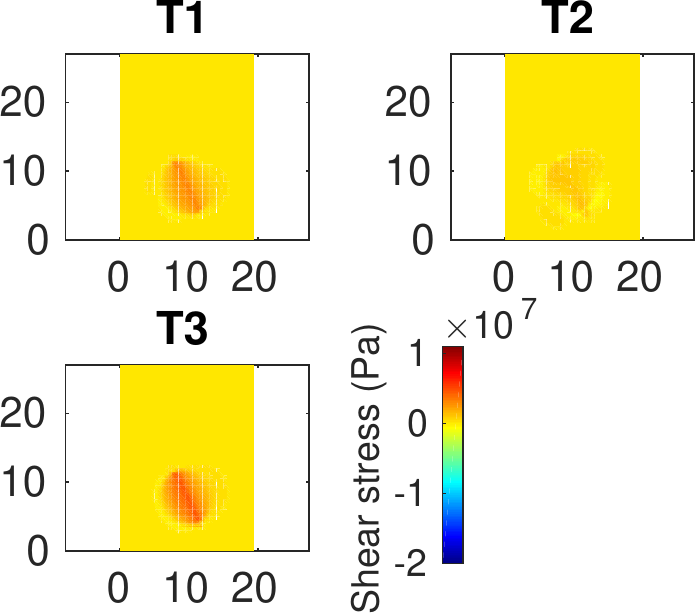
\includegraphics[width=0.8\textwidth]{images/horizontal_00031}
 
\end{frame}

\begin{frame}
 {Shear stress}
 
 \centering \Large T = 3 s\\
 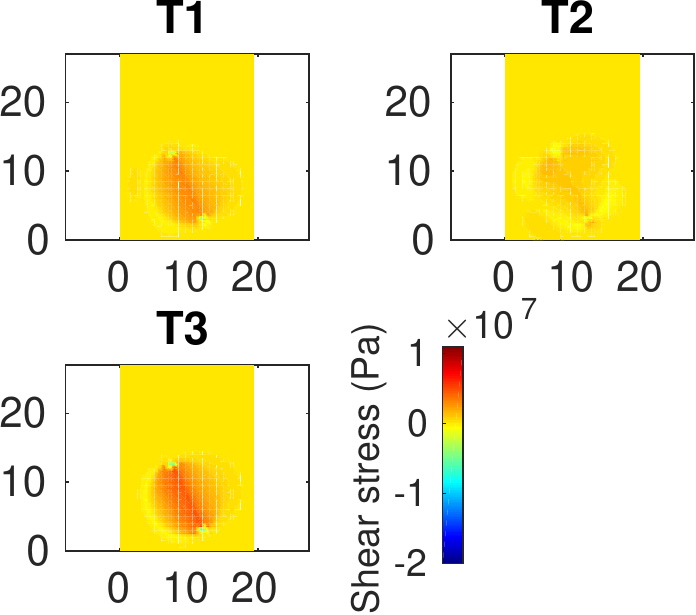
\includegraphics[width=0.8\textwidth]{images/horizontal_00036}
 
\end{frame}

\begin{frame}
 {Shear stress}
 
 \centering \Large T = 3.5 s\\
 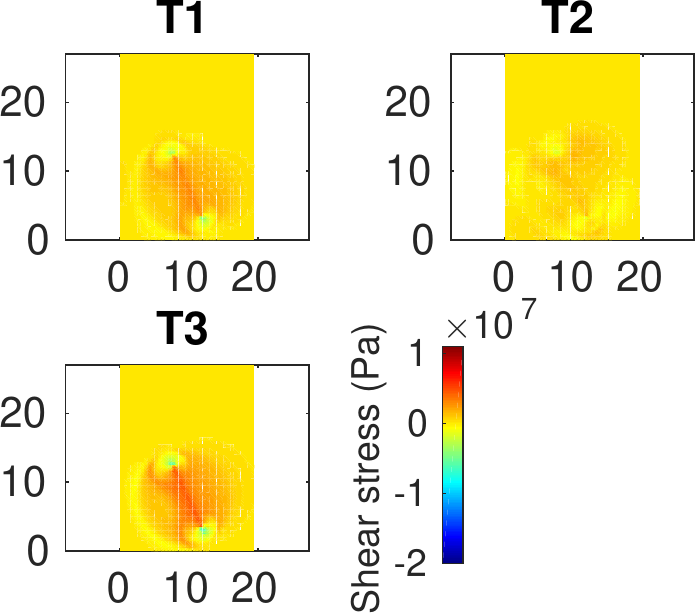
\includegraphics[width=0.8\textwidth]{images/horizontal_00041}
 
\end{frame}

\begin{frame}
 {Shear stress}
 
 \centering \Large T = 4 s\\
 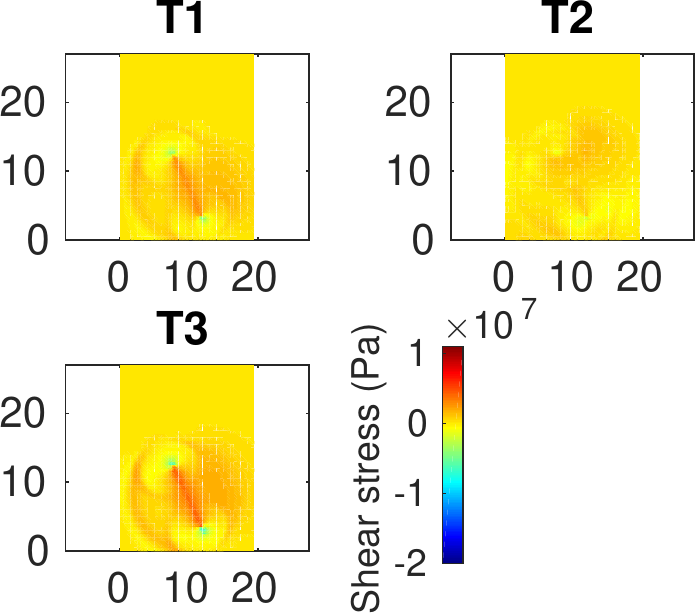
\includegraphics[width=0.8\textwidth]{images/horizontal_00046}
 
\end{frame}

\begin{frame}
 {Shear stress}
 
 \centering \Large T = 4.5 s\\
 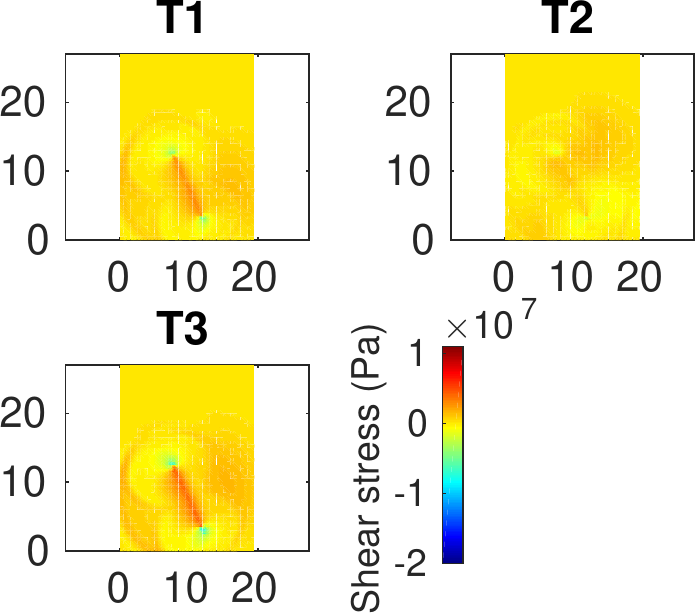
\includegraphics[width=0.8\textwidth]{images/horizontal_00051}
 
\end{frame}

\begin{frame}
 {Shear stress}
 
 \centering \Large T = 5 s\\
 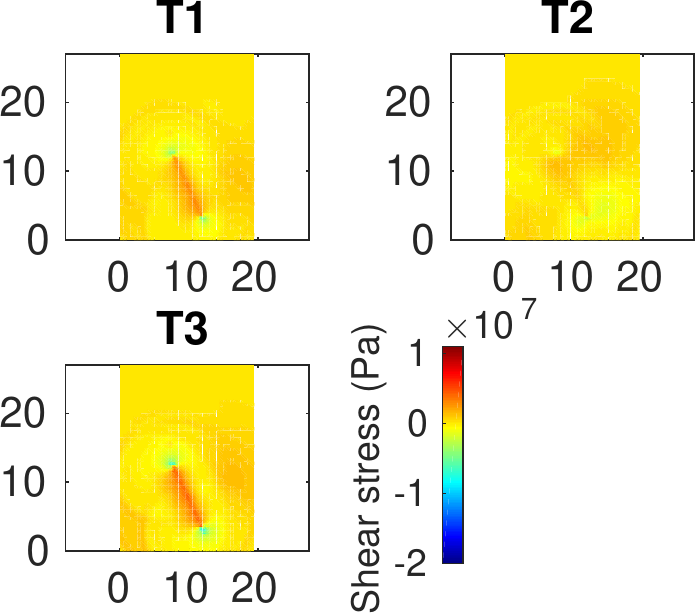
\includegraphics[width=0.8\textwidth]{images/horizontal_00056}
 
\end{frame}

\begin{frame}
 {Shear stress}
 
 \centering \Large T = 5.5 s\\
 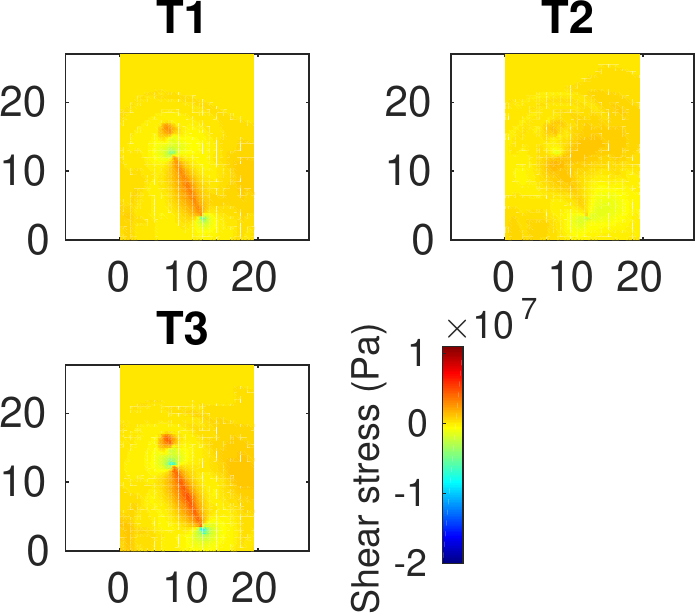
\includegraphics[width=0.8\textwidth]{images/horizontal_00061}
 
\end{frame}

\begin{frame}
 {Shear stress}
 
 \centering \Large T = 6 s\\
 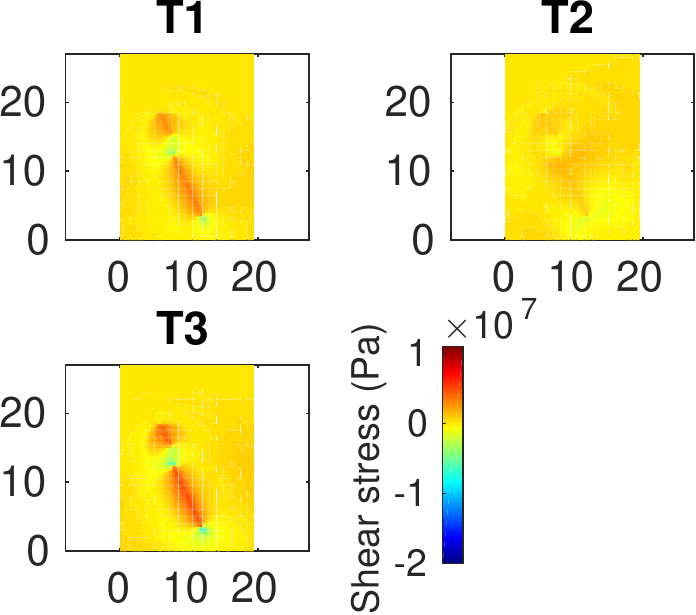
\includegraphics[width=0.8\textwidth]{images/horizontal_00066}
 
\end{frame}

\begin{frame}
 {Shear stress}
 
 \centering \Large T = 6.5 s\\
 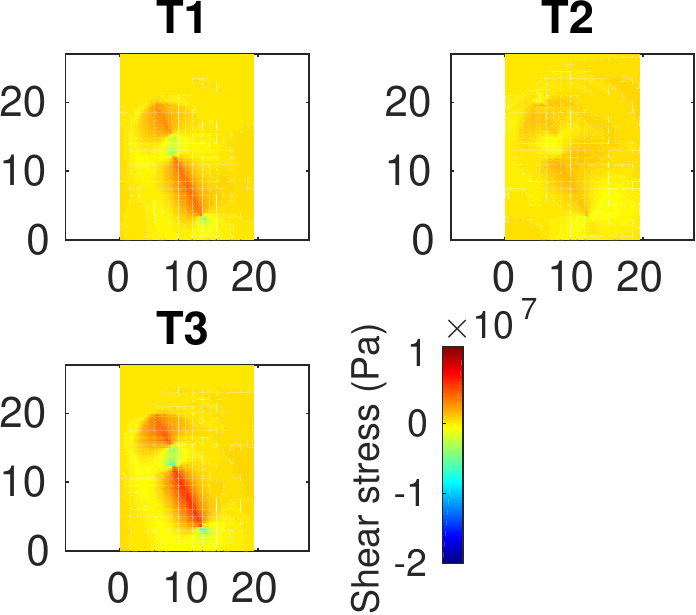
\includegraphics[width=0.8\textwidth]{images/horizontal_00071}
 
\end{frame}

\begin{frame}
 {Shear stress}
 
 \centering \Large T = 7 s\\
 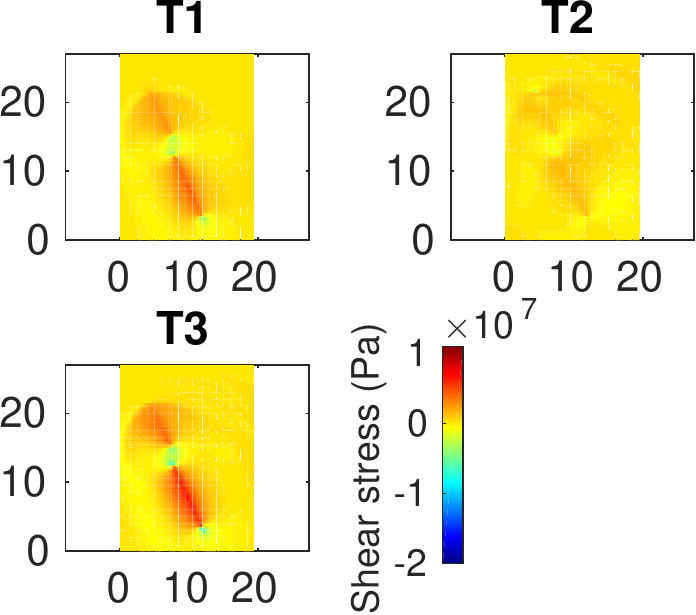
\includegraphics[width=0.8\textwidth]{images/horizontal_00076}
 
\end{frame}

\begin{frame}
 {Shear stress}
 
 \centering \Large T = 7.5 s\\
 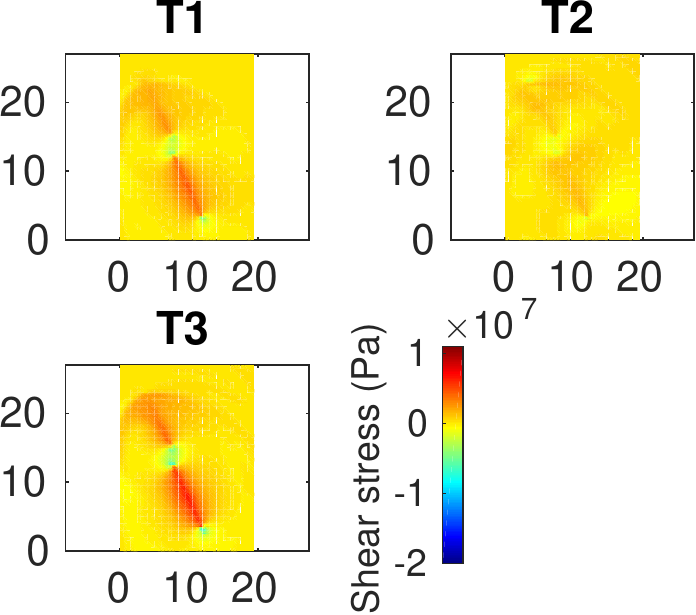
\includegraphics[width=0.8\textwidth]{images/horizontal_00081}
 
\end{frame}

\begin{frame}
 {Shear stress}
 
 \centering \Large T = 8 s\\
 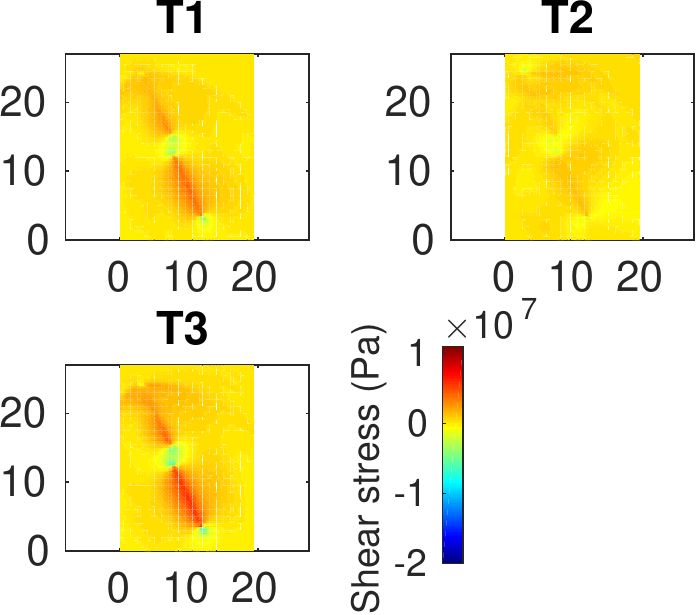
\includegraphics[width=0.8\textwidth]{images/horizontal_00086}
 
\end{frame}

\begin{frame}
 {Shear stress}
 
 \centering \Large T = 8.5 s\\
 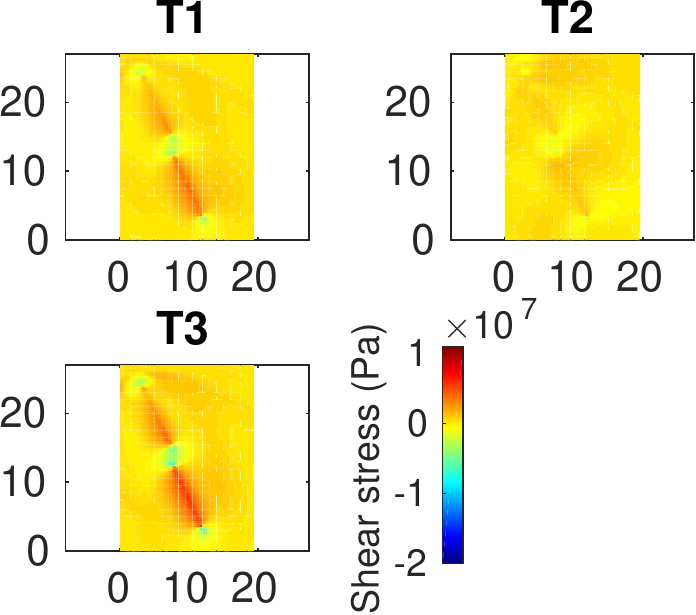
\includegraphics[width=0.8\textwidth]{images/horizontal_00091}
 
\end{frame}

\begin{frame}
 {Shear stress}
 
 \centering \Large T = 9 s\\
 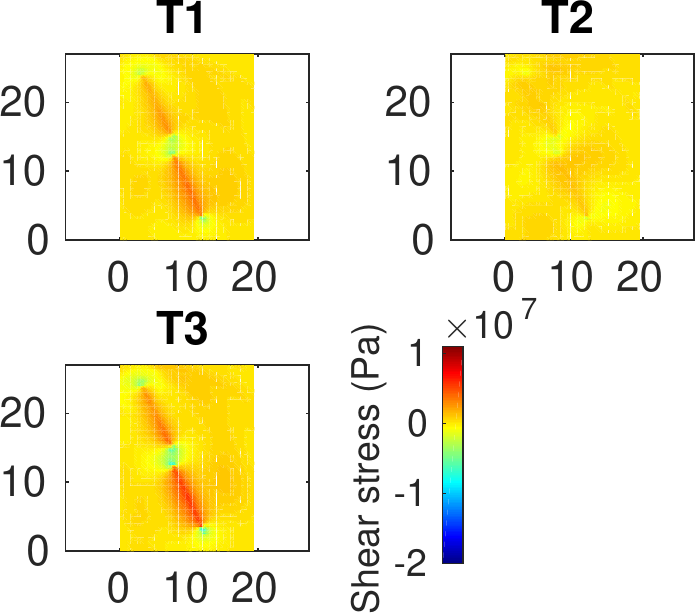
\includegraphics[width=0.8\textwidth]{images/horizontal_00096}
 
\end{frame}

\begin{frame}
 {Shear stress}
 
 \centering \Large T = 9.5 s\\
 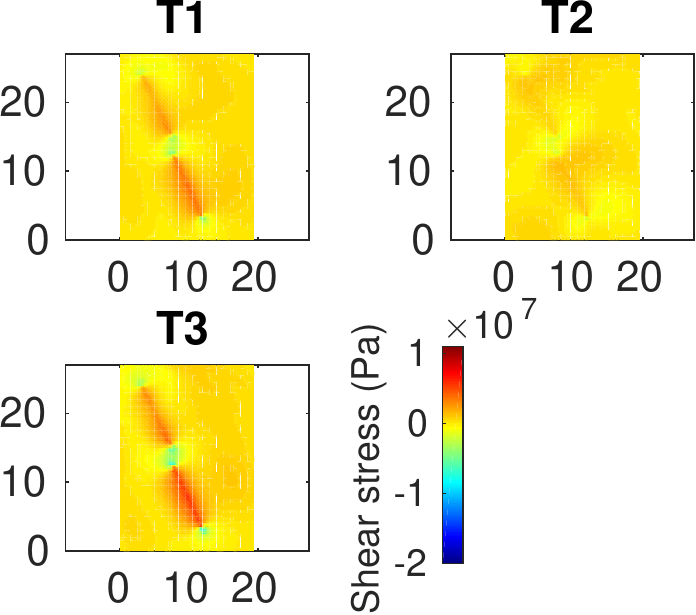
\includegraphics[width=0.8\textwidth]{images/horizontal_00101}
 
\end{frame}

\begin{frame}
 {Shear stress}
 
 \centering \Large T = 10 s\\
 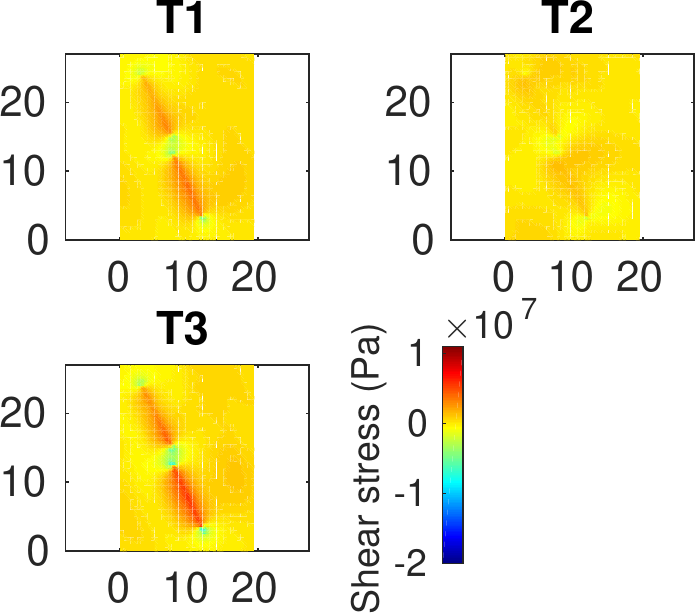
\includegraphics[width=0.8\textwidth]{images/horizontal_00106}
 
\end{frame}

\begin{frame}
 {Shear stress}
 
 \centering \Large T = 10.5 s\\
 \includegraphics[width=0.8\textwidth]{images/horizontal_00111}
 
\end{frame}

\begin{frame}
 {Shear stress}
 
 \centering \Large T = 11 s\\
 \includegraphics[width=0.8\textwidth]{images/horizontal_00116}
 
\end{frame}




\begin{frame}
 {Particle velocity}
 
 \centering \Large T = 0 s\\
 \includegraphics[width=0.8\textwidth]{images/horizontal_velo_00006}
 
\end{frame}

\begin{frame}
 {Particle velocity}
 
 \centering \Large T = 0.5 s\\
 \includegraphics[width=0.8\textwidth]{images/horizontal_velo_00011}
 
\end{frame}

\begin{frame}
 {Particle velocity}
 
 \centering \Large T = 1 s\\
 \includegraphics[width=0.8\textwidth]{images/horizontal_velo_00016}
 
\end{frame}

\begin{frame}
 {Particle velocity}
 
 \centering \Large T = 1.5 s\\
 \includegraphics[width=0.8\textwidth]{images/horizontal_velo_00021}
 
\end{frame}

\begin{frame}
 {Particle velocity}
 
 \centering \Large T = 2 s\\
 \includegraphics[width=0.8\textwidth]{images/horizontal_velo_00026}
 
\end{frame}

\begin{frame}
 {Particle velocity}
 
 \centering \Large T = 2.5 s\\
 \includegraphics[width=0.8\textwidth]{images/horizontal_velo_00031}
 
\end{frame}

\begin{frame}
 {Particle velocity}
 
 \centering \Large T = 3 s\\
 \includegraphics[width=0.8\textwidth]{images/horizontal_velo_00036}
 
\end{frame}

\begin{frame}
 {Particle velocity}
 
 \centering \Large T = 3.5 s\\
 \includegraphics[width=0.8\textwidth]{images/horizontal_velo_00041}
 
\end{frame}

\begin{frame}
 {Particle velocity}
 
 \centering \Large T = 4 s\\
 \includegraphics[width=0.8\textwidth]{images/horizontal_velo_00046}
 
\end{frame}

\begin{frame}
 {Particle velocity}
 
 \centering \Large T = 4.5 s\\
 \includegraphics[width=0.8\textwidth]{images/horizontal_velo_00051}
 
\end{frame}

\begin{frame}
 {Particle velocity}
 
 \centering \Large T = 5 s\\
 \includegraphics[width=0.8\textwidth]{images/horizontal_velo_00056}
 
\end{frame}

\begin{frame}
 {Particle velocity}
 
 \centering \Large T = 5.5 s\\
 \includegraphics[width=0.8\textwidth]{images/horizontal_velo_00061}
 
\end{frame}

\begin{frame}
 {Particle velocity}
 
 \centering \Large T = 6 s\\
 \includegraphics[width=0.8\textwidth]{images/horizontal_velo_00066}
 
\end{frame}

\begin{frame}
 {Particle velocity}
 
 \centering \Large T = 6.5 s\\
 \includegraphics[width=0.8\textwidth]{images/horizontal_velo_00071}
 
\end{frame}

\begin{frame}
 {Particle velocity}
 
 \centering \Large T = 7 s\\
 \includegraphics[width=0.8\textwidth]{images/horizontal_velo_00076}
 
\end{frame}

\begin{frame}
 {Particle velocity}
 
 \centering \Large T = 7.5 s\\
 \includegraphics[width=0.8\textwidth]{images/horizontal_velo_00081}
 
\end{frame}

\begin{frame}
 {Particle velocity}
 
 \centering \Large T = 8 s\\
 \includegraphics[width=0.8\textwidth]{images/horizontal_velo_00086}
 
\end{frame}

\begin{frame}
 {Particle velocity}
 
 \centering \Large T = 8.5 s\\
 \includegraphics[width=0.8\textwidth]{images/horizontal_velo_00091}
 
\end{frame}

\begin{frame}
 {Particle velocity}
 
 \centering \Large T = 9 s\\
 \includegraphics[width=0.8\textwidth]{images/horizontal_velo_00096}
 
\end{frame}

\begin{frame}
 {Particle velocity}
 
 \centering \Large T = 9.5 s\\
 \includegraphics[width=0.8\textwidth]{images/horizontal_velo_00101}
 
\end{frame}

\begin{frame}
 {Particle velocity}
 
 \centering \Large T = 10 s\\
 \includegraphics[width=0.8\textwidth]{images/horizontal_velo_00106}
 
\end{frame}

\begin{frame}
 {Particle velocity}
 
 \centering \Large T = 10.5 s\\
 \includegraphics[width=0.8\textwidth]{images/horizontal_velo_00111}
 
\end{frame}

\begin{frame}
 {Particle velocity}
 
 \centering \Large T = 11 s\\
 \includegraphics[width=0.8\textwidth]{images/horizontal_velo_00116}
 
\end{frame}


\end{document}

